% latex packages to load.
\documentclass[12pt]{article}
\usepackage{geometry}
\geometry{a4paper}
%\geometry{landscape}
\usepackage[parfill]{parskip}    % Activate to begin paragraphs with an empty line rather than an indent
\usepackage{graphicx}
\usepackage{amssymb}
\usepackage{epstopdf}
\usepackage{courier}
\usepackage{fancyhdr}
\usepackage{fullpage}
\usepackage{appendix}
\usepackage{newclude}
\usepackage{datetime}
\usepackage{hyperref}
\usepackage{color}
\usepackage{multicol}
\usepackage{tabularx}
\usepackage{longtable}
\usepackage{enumerate}
\usepackage{enumitem}
\usepackage{listings}
\usepackage{wallpaper}
\usepackage{lastpage}
\usepackage{titling}
\usepackage{multind}
\usepackage[table]{xcolor}
\usepackage{mathtools}

\usepackage{tikz}
\usetikzlibrary{shapes,arrows}

\tikzstyle{block} = [rectangle, draw, text width = 6em, text centered, rounded corners, minimum height = 4em]
\tikzstyle{inputblock} = [rectangle, draw, text width = 24em, minimum height = 2.5em]
\tikzstyle{autographblock} = [rectangle, draw, fill = black!1, text height = 0, text depth = 2cm,text width = 24em, minimum height = 8em]
\tikzstyle{cloud} = [ellipse, draw, minimum height = 4em]
\tikzstyle{line} = [draw, -latex']

% INDEXES
\makeindex{modules}
\newcommand{\usemodule}[1]{\index{modules}{#1}\texttt{#1}}

\definecolor{gray}{rgb}{0.5,0.5,0.5}
\definecolor{tableheader}{rgb}{0.7,0.7,0.7}

\setlist[description]{style=nextline}
\renewcommand{\familydefault}{\sfdefault}

% link setup
\hypersetup{
    colorlinks,
    citecolor=black,
    filecolor=black,
    linkcolor=black,
    urlcolor=black,
}

\DeclareGraphicsRule{.tif}{png}{.png}{`convert #1 `dirname #1`/`basename #1 .tif`.png}

% usefull commands:
\newcommand{\seeref}[1]{\ref{#1} p.\pageref{#1}}
\newcommand{\seeone}[1]{ (zie \ref{#1} p.\pageref{#1})}
\newcommand{\seeonec}[1]{, zie \ref{#1} p.\pageref{#1}}
\newcommand{\seesee}[2]{ (zie \ref{#1} p.\pageref{#1},  \ref{#2} p.\pageref{#2})}

% style for code blocks
\lstset{
    linewidth=1\textwidth,
    breaklines=true,
    numbers=left,                   % where to put the line-numbers
    numberstyle=\tiny\color{gray},  % the style that is used for the line-numbers
    stepnumber=1,                   % the step between two line-numbers. If it's 1, each line 
    numbersep=5pt, 
    basicstyle=\ttfamily\footnotesize,
}

% Header and Footer settings
%\URCornerWallPaper{0.13}{img/dop/koptekstlogo.png}
\pagestyle{fancy}
\fancyhead{}
\renewcommand{\headrulewidth}{0pt}


\fancyfoot[L]{Technisch ontwerp - \projectname}
\fancyfoot[C]{}
\fancyfoot[R]{\textbf{\thepage}\ / \pageref{LastPage}}

% Settings for table of contents.	
\setcounter{secnumdepth}{4}
\setcounter{tocdepth}{3}


\makeatletter
% some extra spacing for the table of contents
\renewcommand{\l@subsection}{\@dottedtocline{2}{1.5em}{3em}}
\renewcommand{\l@subsubsection}{\@dottedtocline{2}{2.7em}{4em}}

\renewcommand\paragraph{%
   \@startsection{paragraph}{4}{0mm}%
      {-\baselineskip}%
      {.5\baselineskip}%
      {\normalfont\normalsize\bfseries}}
\makeatother

% Define variables	
\newcommand{\customer}{Dimpact}
\newcommand{\projectname}{SduConnect}
\newcommand{\thecustomer}{\customer }
\newcommand{\customerdomain}{gemeente.nl}
\newcommand{\customerdomainfull}{http://www.gemeente.nl}
\newcommand{\customerdomainuc}{Gemeente.nl}
\newcommand{\authors}{ Maurits Lawende }


% Voorblad of the documentq
\ThisLRCornerWallPaper{0.8}{img/dop/voorbladlogo.png}

\title{\textbf{\projectname} \\ Technisch Ontwerp}
\pretitle{\begin{flushleft}\LARGE}
\posttitle{\par\end{flushleft}}

\author{}  % skippen we voor maketitle
\date{}

% The actual Document:
\begin{document}
\clearpage \maketitle
 \thispagestyle{empty}
 \vspace{-2.6cm}
  \begin{flushright}
      \ThisLRCornerWallPaper{0.8}{img/dop/voorbladlogo.png}

  \maketitle
 \vspace{-2.6cm}
  \begin{flushright}
\begin{tabularx}{4.6cm}{ X }
Dutch Open Projects         \\
Doornseweg 12                   \\  
3832 RL Leusden                 \\
T: +31[0]33 - 4 50 50 50        \\
F: +31[0]33 - 4 50 50 57        
\\*
\\*
\\*
\\*
\\*
\\*
\\*
\\*
\\*
\\*
\\*
\\*
\\*
\\*
\\*
\\*
\\*
\\*
\\*
\\*



\footnotesize
\copyright All rights reserved.         \\*
\footnotesize
No part of the contents of this publication may be reproduced, stored in a data processing system or transmitted in any form or by any means without the written permission of Dutch Open Projects B.V.

\end{tabularx}
\end{flushright}

\begin{tabularx}{\linewidth}{ p{3cm} X }
  Plaats & Leusden                                \\
  Laatst bijgewerkt & \ddmmyyyydate \today        \\
  Auteurs & \authors                          \\
  Versie & \version                                    \\
\end{tabularx}
\pagebreak



  \end{flushright}
  
 \null
 \vfill    
  \begin{tabularx}{\linewidth}{ p{3cm} X }
    Plaats & Leusden                                                           \\
    Laatst bijgewerkt & \ddmmyyyydate \today           \\
    Auteurs & \authors                                                 \\
    Versie & 1.0                                                                       \\
  \end{tabularx}
\pagebreak

%\section{Beheer}

\begin{tabularx}{\linewidth}{| p{2.5cm} | p{2.5cm} | X | p{2.5cm} |}
\rowcolor{tableheader}
\hline
\textbf{Versie} & \textbf{Datum} & \textbf{Omschrijving} &  \textbf{Auteur}			\\ \hline
0.1 & 17-12-2012 & Draft 											& DOP			\\ \hline
0.2 & 20-12-2012 & Inventarisatie deeloplevering 						& DOP			\\ \hline
0.3 & 08-01-2013 & Toevoeging: cookies, sms, rollen rechten, todo's					& DOP			\\ \hline
0.9 & 09-01-2013 & Toevoeging: HR, gebruikersrollen, persmissieoverzicht & DOP \\ \hline
1.0 & 14-03-2013 & Feedback H. Morang verwerkt & DOP \\ \hline
1.1 & 25-03-2013 & Feedback H. Morang, B. Ot, M. Welleman, J. Zigerman & DOP\\ \hline
1.2 & 29-04-2013 & Feedback H. Morang (punt 1,3,4) & DOP\\ \hline
%versie & datum & omschrijving & auteur             	\\ \hline
\end{tabularx}

\subsection{Akkoord}
Voor akkoord:\\ \\
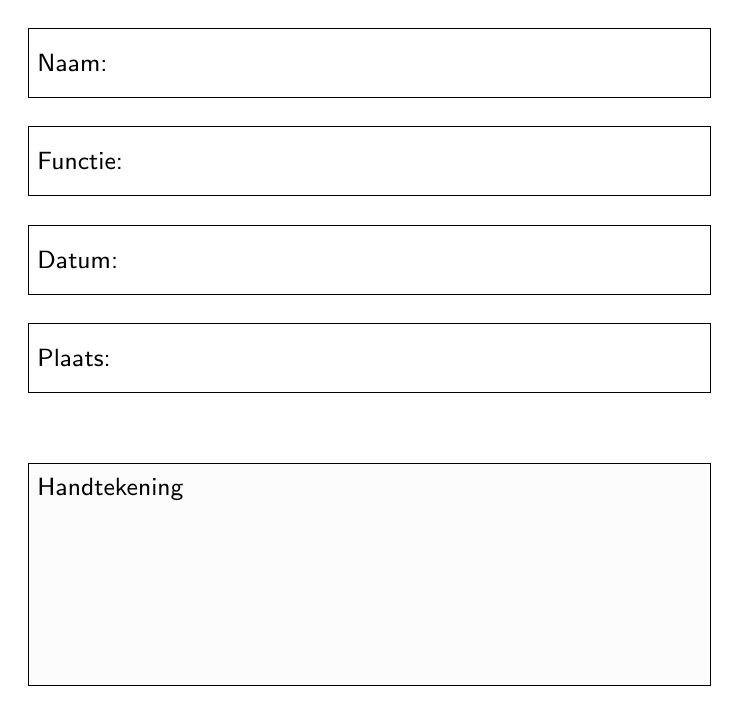
\begin{tikzpicture}
\tikzstyle{every node}=[font=\small];
\node [inputblock] (names) {Naam:};
\node [inputblock, below of = names, node distance = 1.25cm] (function) {Functie:};
\node [inputblock, below of = function, node distance = 1.25cm] (dates) {Datum:};
\node [inputblock, below of = dates, node distance = 1.25cm] (place) {Plaats:};
\node [autographblock, below of = place, node distance = 2.75cm] (autograph) {Handtekening};
\end{tikzpicture}



% table of contents
\renewcommand*\contentsname{Inhoudsopgave}
\tableofcontents

\pagebreak


% The document

\section{Abstract}

Voor Dimpact wordt een nieuwe module ontwikkeld voor de import van PDC en VAC's vanuit de SDU catalogus. Er wordt gebruik gemaakt van de \emph{SduConnect} dienst waarin ook de \emph{SDU Vind} catalogus is ontsloten. Deze module voorziet in een periodieke (incrementele) import.

De nieuw te ontwikkelen functionaliteit wordt onderdeel van de Dimpact Drupal distributie ("WIM"). De module wordt toegevoegd aan het versiebeheer van WIM (in GIT) en gaat mee in bijbehorende release-cycle.

\section{Importmodule}

De import wordt uitgewerkt in een Drupal module onder de naam \texttt{sduconnect}.
De module is in staat om te controleren op updates en deze vervolgens te verwerken. Dit gebeurt zowel automatisch via de cron als handmatig via een button in de admin interface. Tevens kan een bulk-import worden gedaan van alle items.

\subsection{Configuratie}\label{configuratie}

Op \texttt{admin/config/content/sduconnect} wordt een configuratiepagina aangemaakt. Hier wordt een accountnummer ingesteld en worden collecties toegevoegd. Per collectie zijn de volgende instellingen beschikbaar:

\begin{itemize}
\item Collectie id
\item Type: pdc / vac (dropdown)
\item Importfrequentie: uitgeschakeld, 3, 6, 12 of 24 uur (dropdown)
\item Publicatiedomeinen (checkboxes)
\item Onderwaterantwoord importeren (checkbox)
\end{itemize}

De importfrequentie heeft een range van 3 tot 24 uur. Technisch gezien is het mogelijk om vaker te importeren. Het aantal bevragingen van de API is echter onderhevig aan een 'fair use policy', waarbij SDU aangeeft dat ze eens per 3 uur als maximum hanteren. Met de optie "uitgeschakeld" worden geen automatische imports gestart, maar kan wel een handmatige import worden gestart.

\clearpage
\subsection{Importproces}\label{importproces}

De import bestaat uit twee delen, overeenkomstig met de structuur van de SDU API.
\begin{enumerate}
\item Delta service; haalt een lijst op van nieuwe, bijgewerkte en verwijderde items
\item Single item service; haalt \'{e}\'{e}n enkel item op en verwerkt deze in de website
\end{enumerate}

Het eerste onderdeel wordt opgestart in de Drupal cron (via de normale \texttt{hook\_cron}-implementatie) of na het klikken op de button voor een handmatige import. Alle te verwerken items worden in een \emph{queue} gezet. Hiervoor wordt de queue-functionaliteit uit Drupal core gebruikt. De queue items worden ook verwerkt in de cron (via \texttt{hook\_cron\_queue\_info}). Voor nieuwe en bijgewerkte items wordt het item met de "single item service" opgehaald. De inhoud wordt daarna omzet naar een Drupal node en als zodanig opgeslagen. In de database wordt een mapping bijgehouden van id's uit SDU en Drupal node id's.

Bij het ophalen van de nieuwe, bijgewerkte en verwijderde items wordt een startdatum meegegeven. Hiervoor wordt de \emph{servertime} uit de response van de voorgaande aanroep gebruikt. Deze datum geeft aan tot welk tijdstip de wijzigingen nog in de response zijn meegenomen. Deze datum wordt in de database opgeslagen \emph{per collectie}.

\subsubsection{Bulk import}

Na het aanmaken van een nieuwe collectie is de \emph{servertime} van de laatste import nog niet beschikbaar. In dit geval worden alle beschikbare items ge\"{i}mporteerd. Technisch worden hiervoor dezelfde processen gebruikt, maar worden alle opdates sinds datum "0000-00-00" opgevraagd bij de API. Dit is een \'{e}\'{e}nmalig proces.

\subsubsection{Wekelijkse correctie}

Eens per week worden de updates van de afgelopen 7 dagen opgevraagd, in plaats van sinds de vorige update. Hiermee worden eventuele niet doorgevoerde updates alsnog verwerkt. Dit is een aanbeveling uit de SduConnect implementatiehandleiding.
De volledige update wordt gedaan wanneer de import draait op zondag en de \texttt{servertime} op de dag ervoor staat. Met andere woorden; iedere zondag (bij de eerste sync) worden alle updates van de afgelopen week verwerkt.

\subsubsection{Foutafhandeling}

Wanneer de API niet bereikbaar is wordt daar altijd melding van gemaakt in de log\seeone{logging}.
Als het om de \emph{delta service} gaat dan wordt dit verder genegeerd. Een tweede poging wordt automatisch gedaan in de volgende cron run.
De items zelf worden altijd verwerkt als apart \emph{queue item}. Wanneer de API niet beschikbaar is dan wordt een \emph{Exception} gegeven. De cron pakt dit op en laat daarop het item in de queue staan. Deze wordt dan na een uur opnieuw uitgevoerd.

\subsection{Handmatige import}

De handmatige import start de delta-import\seeone{importproces} na het klikken op een button in de admin-interface. De gebruiker krijgt te zien hoeveel items bijgewerkt, nieuw en verwijderd zijn. De items worden via de gebruikelijke weg verwerkt (in cron). In de interface is het aantal items in de queue te zien, waarmee men kan controleren of de import is voltooid.

\subsection{Statistieken}

Op de configuratiepagina wordt het aantal items in de queue getoond. Deze wordt uitgelezen uit de \texttt{queue}-tabel. Daarnaast is per collectie de "bijgewerkt tot" datum te zien en het aantal ge\"{i}mporteerde items.

\clearpage
\subsection{Logging}\label{logging}

Onder een aparte tab op de configuratiepagina is een lijst te zien van logberichten. Een logbericht bevat de volgende informatie:
\begin{itemize}
\item Datum en tijd
\item Type
\item Verwijzing naar node (titel met hyperlink)
\item Verwijzing naar XML
\end{itemize}

De volgende types zijn mogelijk:
\begin{enumerate}\label{logtypes}
\item API onbereikbaar
\item Nieuw item
\item Nieuw item (niet gevonden)
\item Bijgewerkt item
\item Bijgewerkt item (niet gevonden)
\item Verwijderd item
\item Verwijderd item (niet gevonden)
\end{enumerate}

De "niet gevonden" statussen kunnen twee oorzaken hebben; het item komt terug uit de \emph{delta service} maar niet uit de \emph{single item service} (bij nieuwe of bijgewerkte items) of; het item is niet gevonden als Drupal node (bij bijgewerkte of verwijderde items). De "niet gevonden" status duidt niet altijd op een fout. Er kunnen valide oorzaken zijn zoals het aanmaken \'{e}n verwijderen van hetzelfde item tussen twee imports in.

De verwijzing naar de XML is altijd een link naar het pad \texttt{node/\%/sduconnect-xml}. Dit is alleen van toepassing bij nieuwe en bijgewerkte items. Deze functie kan gebruikt worden voor testdoeleinden. Op dit pad staat een callback die de XML ophaalt van de SDU API en vervolgens teruggeeft aan de browser. Er wordt niet direct verwezen naar de SDU API omdat die URL mogelijk niet bezocht kan worden vanwege IP-restricties.

\subsection{Permissies}

Er worden twee permissies aangemaakt.

\begin{itemize}
\item \texttt{administer sduconnect module} \\
  Wijzigingen van instellingen en beheren van collecties.
\item \texttt{view sduconnect info} \\
  Statistieken bekijken en handmatige import starten.
\end{itemize}

\clearpage
\section{Samenwerkende catalogi feed}

De export voor \emph{samenwerkende catalogi} wordt uitgewerkt in een afzonderlijke module onder de naam \texttt{scfeed}. Deze module biedt een callback aan op het pad \texttt{/sc-feed} waarop een XML feed te vinden is van producten in IPM 4.0 formaat\footnote{http://standaarden.overheid.nl/sc}. Alle nodes van het type \texttt{product} die gepubliceerd zijn op het domein waarop de feed wordt aangeroepen komen in de output.
Er is geen afhankelijkheid naar de \texttt{sduconnect}-module. De \texttt{scfeed} module kan daarom ook worden gebruikt zonder gebruik te maken van de SDU import. Er is wel een afhankelijkheid naar het \texttt{product} nodetype en bijbehorende velden.

Bij het opslaan en toevoegen van items zal deze module de XML codes per product genereren m.b.v. \emph{queue items} (via \texttt{hook\_cron\_queue\_info}. De voorgedefini\"{e}erde XML snippets worden dan in de database opgeslagen, zodat later snel een volledige feed samengesteld kan worden.

\subsection{Configuratie}

Er wordt een settings-pagina gemaakt met de volgende opties:
\begin{itemize}
\item Instellen van uitgever \\
Dit is een verplicht veld in de XML. Met een dropdown kan een waarde worden opgegeven die aangeeft van welke gemeente de informatie afkomstig is. Deze waarde moeten beschikbaar zijn in de lijsten die de standaard voorschrijft\footnote{http://standaarden.overheid.nl/owms/terms/Gemeente.xml}. De lijst van gemeenten wordt als XML opgenomen in de module, zodat deze opties in de interface beschikbaar zijn. Deze informatie wordt niet automatisch bijgewerkt aangezien hier geen vastgestelde API voor beschikbaar is. Dit vormt enkel een probleem wanneer na een gemeentelijke herindeling een nieuwe gemeente gebruik gaat maken van deze module. In dat geval kan een nieuwe XML van de overheids-website worden opgehaald en in de module worden gezet.  
\item Hergenereren van XML-data \\
Hiermee wordt de huidige data weggegooid en worden queue items aangemaakt voor alle nodes van het type \texttt{product}.
\end{itemize}

Het proces om de XML te hergenereren wordt ook uitgevoerd in een \texttt{hook\_enable}-implementatie. Daardoor wordt de data ook gegenereerd na het aanzetten van deze module - voor reeds bestaande producten.

\clearpage
\appendix
\appendixpage\label{appendices}
\addappheadtotoc


\section{VAC velden}
Bestaande velden:
\begin{itemize}
\item Titel \\ De vraag wordt gebruikt als titel van de node.
\item Body \\
De volgende vrije tekstvelden worden ge\"{i}mporteerd als onderdeel van de \emph{node body}:
\begin{itemize}
\item Antwoord tekst
\item Productveld
\item Onderwaterantwoord (alleen indien aangevinkt in configuratie\seeonec{configuratie})
\end{itemize}
De velden worden in bovengenoemde volgende achter elkaar gezet zonder toevoeging van headers of tabs.
\item Toelichting
\item Locatie \\ Bevat het antwoordadres zoals aangegeven in SduConnect.
\item Tags \\ Bevat de doelgroepen en trefwoorden.
\end{itemize}

Nieuwe velden:
\begin{itemize}
\item Meer informatie \\
Type: \texttt{link} \\
Getoond als: lijst met links
\item Relaties naar pdc / vacs \\
Type: \texttt{entity\_reference} \\
Getoond als: lijst met links
\end{itemize}

\clearpage
\section{PDC velden}
Bestaande velden:
\begin{itemize}
\item Titel
\item Body \\
De volgende vrije tekstvelden worden ge\"{i}mporteerd als onderdeel van de \emph{node body}:
\begin{itemize}
\item Omschrijving
\item Let op
\item Voorwaarden
\item Aanpak
\item Termijn
\item Bezwaar en beroep
\item Kosten
\item Contact
\item Indienperiode
\item Beschikbaar budget
\item Maximale bijdrage
\end{itemize}
De velden worden in bovengenoemde volgende achter elkaar gezet. Alle velden met uitzondering van "Omschrijving" en "Let op" komen in een aparte tab.
\item Tags \\
De tags worden gebruikt om de thema's en doelgroepen in te importeren.
\item Datum \\
Start- en einddatum indien aangegeven in SduConnect (dit zijn andere velden dan de publicatiedata).
\item Locatie \\
Bevat het indieningsadres, indien opgegeven in SduConnect.
\end{itemize}

Nieuwe velden:
\begin{itemize}
\item Verwijzingen wetten / regelgeving \\
type: \texttt{link} \\
Getoond als: lijst met links
\item Online aanvragen \\
type: \texttt{link} \\
Getoond als: link
\item Formulieren \\
type: \texttt{link} \\
Getoond als: lijst met links
\item Meer informatie (link) \\
type: \texttt{link} \\
Getoond als: link
\item Relaties naar PDC / VAC's ("Gerelateerd")\\
type: \texttt{link} \\
Getoond als: lijst met links
\item Samenwerkende catalogi doelgroep \\
type: \texttt{text} (checkboxes) \\
Getoond als: \emph{niet}
\end{itemize}

\clearpage
\section{Databasestructuur}

\subsection*{collection}
\begin{tabular}{p{.25\textwidth} | p{.25\textwidth} | p{.5\textwidth} }
\textbf{Kolomnaam} & \textbf{Type} & \textbf{Toelichting} \\
\hline
cid & int & Surrogate key \\
external\_id & int & Collection id bij SDU \\
type & varchar & "pdc" of "vac" \\
name & varchar & Naam van de collectie (enkel getoond in admin) \\
items & int & Aantal items \\
updated\_till & int & Unix timestamp \\
frequency & int & Aantal seconden tussen automatische imports \\
import\_private & int (boolean) & Importeer onderwatervelden
\end{tabular}


\subsection*{collection\_domain}
\begin{tabular}{p{.25\textwidth} | p{.25\textwidth} | p{.5\textwidth} }
\textbf{Kolomnaam} & \textbf{Type} & \textbf{Toelichting} \\
\hline
cid & int & Id van \texttt{collection} \\
domain\_id & int & Id van domain
\end{tabular}

\subsection*{item}
\begin{tabular}{p{.25\textwidth} | p{.25\textwidth} | p{.5\textwidth} }
\textbf{Kolomnaam} & \textbf{Type} & \textbf{Toelichting} \\
\hline
nid & int & Node id \\
cid & int & Id van \texttt{collection} \\
external\_id & int & Id bij SDU
\end{tabular}

\subsection*{log}
\begin{tabular}{p{.25\textwidth} | p{.25\textwidth} | p{.5\textwidth} }
\textbf{Kolomnaam} & \textbf{Type} & \textbf{Toelichting} \\
\hline
lid & int & Surrogate key \\
date & int & Unix timestamp \\
type & int & Type\seeone{logtypes} \\
cid & int & Id van \texttt{collection} \\
nid & int & Node id \\
title & varchar & Node title
\end{tabular}

\end{document}
